\documentclass[compress, 8pt]{beamer}
% \documentclass[handout, 8pt]{beamer}
\usepackage[utf8]{inputenc}

% Notes to self: \nts[color option]{text that is a note}
\newif\ifshowcomments
% \showcommentstrue % uncomment to show


% Standard packages
\usepackage{hyperref} % Include links
\usepackage{setspace} % More control over local line spacing: http://felix11h.github.io/blog/line-spacing-beamer
% Math
\usepackage{amsthm, amsmath, mathtools}
\usepackage{appendixnumberbeamer}
% Multi=row and column
\usepackage{multirow,multicol}
% multiline columns
\usepackage{tabularx}
% bold math symbols
\usepackage{bm}


\usepackage{ifthen}

\usepackage{amsbsy}

%%%%%%%%%%%%%%
% Formatting %
%%%%%%%%%%%%%%

% Outer theme
\useoutertheme[subsection=false]{miniframes}
% Fix to display navigational dots; dots only shown for subsections
% Can comment out to have no dots in presentation
\AtBeginSection[]{\subsection{}}
% Font
\usepackage[default]{cantarell}

% Colors
\usepackage{xcolor}
% UCSD color palette: http://ucpa.ucsd.edu/brand/elements/color-palette/
\definecolor{DarkBlue}{RGB}{24, 43, 73}
\definecolor{MainBlue}{RGB}{0, 106, 150}
\definecolor{LightBlue}{RGB}{0, 198, 215}
\definecolor{Green}{RGB}{110 150 59}
\definecolor{Yellow}{RGB}{255 205 0}
\definecolor{LightYellow}{RGB}{243 29 0}
\definecolor{Gold}{RGB}{198 146 20}
\definecolor{Orange}{RGB}{252 137 0}
\definecolor{LightGrey}{RGB}{182, 177, 169}
\definecolor{DarkGray}{RGB}{116 118 120}
\definecolor{DarkPurple}{RGB}{25 0 51}
\definecolor{Purple}{RGB}{55 24 81}
\definecolor{Maroon}{HTML}{6A123D}
\definecolor{HunterPurple}{HTML}{5F259F}
\definecolor{HunterGold}{HTML}{FFC72A}
\definecolor{HunterGray}{HTML}{EEECF0}


% Hyperlink colors
\hypersetup{
  colorlinks   = true, %Colours links instead of ugly boxes
  urlcolor     = Maroon, %Colour for external hyperlinks
  linkcolor    = DarkGray, %Colour of internal links
  citecolor   = HunterPurple %Colour of citations
}


% Learned using: https://ramblingacademic.com/2015/12/how-to-quickly-overhaul-beamer-colors/
% To change additional sections: http://www.cpt.univ-mrs.fr/~masson/latex/Beamer-appearance-cheat-sheet.pdf
\setbeamercolor{palette primary}{bg=HunterPurple,fg=white}
\setbeamercolor{palette secondary}{bg=HunterPurple,fg=white}
\setbeamercolor{palette tertiary}{bg=HunterPurple,fg=white}
\setbeamercolor{palette quaternary}{bg=HunterPurple,fg=white}
\setbeamercolor{structure}{fg=HunterPurple} % itemize, enumerate, etc
\setbeamercolor{section in toc}{fg=HunterPurple} % TOC sections
\setbeamercolor{section in head/foot}{bg=HunterPurple,fg=LightGrey}
%\setbeamercolor{navigation symbols}{bg=Gold, fg=Gold}
\setbeamercolor{alerted text}{fg=MainBlue}
\beamertemplatenavigationsymbolsempty
%tem
%\setbeamertemplate{itemize items}

% Make bullet size smaller
\setbeamertemplate{itemize item}{\tiny\raise1.4pt\hbox{$\blacktriangleright$}}
\setbeamertemplate{itemize subitem}{--}
% make bullet closer to the text
\setlength{\labelsep}{.8ex}

% get rid of 'Figure: ' in caption
\setbeamertemplate{caption}{\raggedright\insertcaption\par}
% Caption flushed left
\usepackage{caption}
\captionsetup{%
    labelformat=empty,
    font=small,
    singlelinecheck=false,
    tableposition=top
}


%%%%%%%%%%%%%%%%
% New commands %
%%%%%%%%%%%%%%%%

\ifshowcomments
\newcommand{\nts}[2][DarkGray]{\setbeamercolor{taras comment}{fg=#1}{\usebeamercolor[fg]{taras comment}\setbeamercolor{item}{fg = taras comment.fg}\emph{#2}}}
\else 
\newcommand{\nts}[2][DarkGray]{}
\fi

% Timed color highlights
\newcommand<>{\blue}[1]{\textbf{\color#2{MainBlue}#1}}
\newcommand<>{\mblue}[1]{{\color#2{MainBlue}#1}}
\newcommand<>{\green}[1]{\textbf{\color#2{Green}#1}}
\newcommand<>{\mgreen}[1]{{\color#2{Green}#1}}

\newcommand{\EE}{\mathbf{E}}
\newcommand{\PP}{\mathbf{P}}
\newcommand{\llog}[1]{\log \left( #1 \right)}
\newcommand{\Cov}[1]{\text{Cov} \left( #1 \right)}
\newcommand{\Var}[1]{\text{Var} \left( #1 \right)}
\newcommand{\XX}{\mathbf{X}}
\newcommand{\xx}{\mathbf{x}}

\newcommand{\br}[1]{\left\{ #1 \right\}}
\newcommand{\sbr}[1]{\left[ #1 \right]}
\newcommand{\pr}[1]{\left( #1 \right)}
\newcommand{\ce}[2]{\left[\left. #1 \right\vert #2 \right]}
\newcommand{\cls}[2]{\left. #1 \right\vert #2}
\newcommand{\crs}[2]{#1 \left\vert #2 \right.}
\newcommand{\ceil}[1]{\left\lceil #1 \right\rceil}

% Beamer buttons
% bottom buttom: \bbutton{name_of_link}{Text to print}
\newcommand{\bbutton}[2]{
    \begin{tikzpicture}[remember picture, overlay]
    \node[shift={(-1.4cm,0.5cm)}]() at (current page.south east){%
    \hyperlink{#1}{\beamergotobutton{#2}}};    
    \end{tikzpicture}
}    
% here button
\newcommand{\hbutton}[2]{
    \hyperlink{#1}{\beamergotobutton{#2}}
}
% Cite command: cc
\newcommand{\nn}[2][DarkGray]{{\small \color{#1} #2}}
\newcommand{\ccdoi}[2]{\href{https://doi.org/#1}{\nn{#2}}}
\newcommand{\ccurl}[2]{\href{#1}{\nn{#2}}}

% change slide width on a single slide
% source: https://tex.stackexchange.com/questions/160825/modifying-margins-for-one-slide/242073
\newcommand\Wider[2][3em]{%
\makebox[\linewidth][c]{%
  \begin{minipage}{\dimexpr\textwidth+#1\relax}
  \raggedright#2
  \end{minipage}%
  }%
}

% To remove sections from appendix
% source: https://tex.stackexchange.com/questions/37127/how-to-remove-some-pages-from-the-navigation-bullets-in-beamer
\makeatletter
\let\beamer@writeslidentry@miniframeson=\beamer@writeslidentry
\def\beamer@writeslidentry@miniframesoff{%
  \expandafter\beamer@ifempty\expandafter{\beamer@framestartpage}{}% does not happen normally
  {%else
    % removed \addtocontents commands
    \clearpage\beamer@notesactions%
  }
}
\newcommand*{\miniframeson}{\let\beamer@writeslidentry=\beamer@writeslidentry@miniframeson}
\newcommand*{\miniframesoff}{\let\beamer@writeslidentry=\beamer@writeslidentry@miniframesoff}
\makeatother

%%%%%%%%%%%%%%%%%%%%
% Figures and tikz %
%%%%%%%%%%%%%%%%%%%%

% \usepackage{pgfplots} % maybe for tikz axes?
\usepackage{graphicx} % Include figures
\usepackage{tikz} % Draw figures with tikz
\usetikzlibrary{positioning} % to use right=of <node> syntax
\usetikzlibrary{shapes} % for other node shapes; see http://www.texample.net/tikz/examples/node-shapes/
% \usetikzlibrary{shapes.multipart} % multiline nodes in tikz
\usetikzlibrary{shapes.arrows} % arrow nodes in tikz
% \usetikzlibrary{shapes.misc} % miscellaneous nodes in tikz; for rounded rectangles
% \usetikzlibrary{shapes.geometric} % geometric nodes in tikz; fortriangles
% \usetikzlibrary{shapes.ellipse} % geometric nodes in tikz; fortriangles
\usetikzlibrary{positioning} % I think this let's you use "right of", "left of"

% Presentation specific tikz
%\usetikzlibrary{tikzmark} % to use tikzmarkto add braces to itemize
% \usetikzlibrary{calc} % for widthof
% \tikzset{
%     above label/.style={
%         above = 5pt,
%         %font=\footnotesize,
%         text height = 1.5ex,
%         text depth = 1ex,
%     },
%     below label/.style={  
%         below=4pt,
%         %font=\footnotesize,
%         text height = 1.5ex,
%         text depth = 1ex
%     },
%     brace label/.style={
%         below = 4pt,
%         font=\footnotesize,
%         text height = 1.5ex,
%         text depth = 1ex
%     },
%     brace/.style={
%         decoration={brace, mirror},
%         decorate
%     }
% }

% For every picture that defines or uses external nodes, you'll have to
% apply the 'remember picture' style. To avoid some typing, we'll apply
% the style to all pictures.
%\tikzstyle{every picture}+=[remember picture]

% To avoid a warning
% \pgfplotsset{compat=1.7}
\usepackage[normalem]{ulem}

%%%%%%%%%%%%%%%%%%%%%%%%%%%%%%%%%%%%%%%%%%%%%%%%%%%%%%%%%%%%%%%%%%%%%%%%%%%%%%
% Paths to figures
\usepackage{subcaption}

% Avoid a warning on mac; can introduce a warning (and maybe a break) on windows
% \usepackage{etex}
% Avoid a warning
\let\Tiny=\tiny

%Information to be included in the title page:
\title{Linear regression + Matching}
\subtitle{ECON726}
\author[]{Tara Sullivan}
\institute{
Tara Sullivan \\
\textit{tara.sullivan55@login.cuny.edu}
}
\date{
\today
\nts{\\
\medskip
Notes/comments are in gray and will be excluded from the presentation.
}
}

% plot graphs with pgfplots
\usepackage{pgfplots}
\pgfplotsset{compat=newest}
\usepgfplotslibrary{groupplots}
\usepgfplotslibrary{dateplot}
\pgfplotsset{compat=newest,
    every axis/.style={
        axis y line*=left,
        axis x line*=bottom,
        % allows for multi-line legend entries
        legend style={cells={align=left}},
        % allows for multi-line titles
        title style={align=center},
    },
}

% For animations using underbrace 
% Source: https://tex.stackexchange.com/a/565866
\usepackage{xparse, letltxmacro}
\LetLtxMacro{\oldunderbrace}{\underbrace}
\DeclareDocumentCommand{\underbrace}{d<> m e{_}}{%
  \IfValueTF{#1}{% IF <overlay-specification> given
    % using global onlside flag, cf. p82 beamer manual v3.59
    \oldunderbrace{#2\onslide<#1>}_{#3}\onslide%
  }{% ELSE
    \oldunderbrace{#2}_{#3}
  }%
}%

\usetikzlibrary{decorations.pathreplacing,calligraphy}

%%%%%%%%%%%%%%%%%%%%%%%%%%%%%%%%%%%%%%%%%%%%%%%%%%%%%%%%%%%%%%%%%%%%%%%%%%%%%%%%
\begin{document}    
%\beamertemplatenavigationsymbolsempty


%%%%%%%%%%%%%%%%%%%%%%%%%%%%%%%%%%%%%%%%%%%%%%%%%%%%%%%%%%%%%%%%%%%%%%%%%%%%%%%%
\begin{frame}
\titlepage
% \tikzset{external/figure name={intro_}}
\end{frame}

%%%%%%%%%%%%%%%%%%%%%%%%%%%%%%%%%%%%%%%%%%%%%%%%%%%%%%%%%%%%%%%%%%%%%%%%%%%%%%%%
\begin{frame}{Housekeeping}

\textbf{Today}
\begin{itemize}
    \item Discuss paper selection
    \item Finish linear regression
    \item Introduction to matching
    \item Review examples in jupyter notebooks
    (\href{https://github.com/tara-sullivan/econ726-notebooks/blob/main/notebooks/04-regression.ipynb}{regression}; \href{https://github.com/tara-sullivan/econ726-notebooks/blob/main/notebooks/05-matching.ipynb}{matching})
\end{itemize}

\vspace{3ex}
\textbf{Homework}
\begin{itemize}
    \item 
\end{itemize}

\end{frame}

%%%%%%%%%%%%%%%%%%%%%%%%%%%%%%%%%%%%%%%%%%%%%%%%%%%%%%%%%%%%%%%%%%%%%%%%%%%%%%%%
\begin{frame}{Empirical project}

    I use negative grading. I'm sorry it seems harsh! You all had great starts to your projects!

    \begin{itemize}
        \item Limitations of data should be meaningful. Who aren't you looking at? 
        \item Does SUTVA apply?
        \item Include your paper title, authors etc. Ideally, also include the link! And ideally, in an appendix, include the original figures you're referencing!
        \item Imagine you are explaining to a coworker who has no idea about the context of your paper. 
    \end{itemize}

\end{frame}

%%%%%%%%%%%%%%%%%%%%%%%%%%%%%%%%%%%%%%%%%%%%%%%%%%%%%%%%%%%%%%%%%%%%%%%%%%%%%%%%
\begin{frame}{Empirical project}

\textbf{Paper selection}: Due \textbf{September 28} [5\% of final grade]
\begin{itemize}
    \item Done!
\end{itemize}

\textbf{Project plan}: Due \textbf{October 13} [15\% of final grade] 
\begin{itemize}
\item Done!
\end{itemize} 

\textbf{Replication results}: Due \textbf{November 2}: [10\% of final grade]
\begin{itemize}
\item You should submit some of your main replication results. The final results should be formatted as tables and charts in a word document or PDF, submitted on Brightspace. Your code and data should accessible on GitHub.
\end{itemize}

\textbf{Presentation}: Due \textbf{December 1} \& \textbf{December 8} [10\% of final grade]
\begin{itemize}
\item Prepare a 10 minute presentation on your paper. Focus on the research question, main result, and one extension. 
\end{itemize}

\textbf{Final Paper}: Due \textbf{December 11} [40\% of final grade]
\begin{itemize}
\item Your paper should contain 6-10 pages of text, and 3-6 pages of figures (double spaced, 12 point font).
You must provide the code and data to replicate your findings. 
Your final project should be submitted on Brightspace, and your code and data should be uploaded to github (note: if your data is too large to upload to github, let me know). 
\end{itemize}

\end{frame}

%%%%%%%%%%%%%%%%%%%%%%%%%%%%%%%%%%%%%%%%%%%%%%%%%%%%%%%%%%%%%%%%%%%%%%%%%%%%%%%
\miniframesoff
\begin{frame}{Outline}
    \tableofcontents
\end{frame}
\miniframeson

%%%%%%%%%%%%%%%%%%%%%%%%%%%%%%%%%%%%%%%%%%%%%%%%%%%%%%%%%%%%%%%%%%%%%%%%%%%%%%%%
\section[Matching]{Matching}
\miniframesoff
\begin{frame}
    \tableofcontents[currentsection]
\end{frame}
\miniframeson
%%%%%%%%%%%%%%%%%%%%%%%%%%%%%%%%%%%%%%%%%%%%%%%%%%%%%%%%%%%%%%%%%%%%%%%%%%%%%%%%

% %%%%%%%%%%%%%%%%%%%%%%%%%%%%%%%%%%%%%%%%%%%%%%%%%%%%%%%%%%%%%%%%%%%%%%%%%%%%%%%%
% \begin{frame}{}



% Linear causal model seems like a strong assumption. How realistic is it to assume that policy responses are linear?
% \begin{itemize}
%     \item Luckily, you don't always need to worry about that to run regressions
%     \item You can think of linear regression of $Y_i$ on $X_i$ and $s_i$ as providing the best \textbf{linear approximation} to the underlying CEF
%     \item 
% \end{itemize}

% \end{frame}

%%%%%%%%%%%%%%%%%%%%%%%%%%%%%%%%%%%%%%%%%%%%%%%%%%%%%%%%%%%%%%%%%%%%%%%%%%%%%%%%
\begin{frame}{Motivating example}

Consider the universe of applicants to the U.S. military:
\begin{itemize}
    \item $Y_i$: average earnings
    \item $D_i$: dummy variable indicating whether $i$ served in the military
\end{itemize}
We may be interested in the average effect of treatment on the treated (ToT):
\begin{equation*}
    \EE [Y_i(1) - Y_{i}(0) \vert D_i = 1]
\end{equation*}
Difference between:
\begin{itemize}
    \item Average earnings of soldiers (observable)
    \item Average earnings of soldiers, had they not served (unobservable)
\end{itemize}
Na{\"i}ve comparisons (average predicted effect) will be biased:
\begin{align*}
\EE [Y_i \vert D_i = 1] - \EE [Y_i \vert D_i=0] 
=& \underbrace{\EE [Y_i(1) - Y_i(0) \vert D_i = 1]}_{\text{ATE on treated}} 
+ \underbrace{\EE [Y_i(0) \vert D_i = 1] - \EE [Y_i(0) \vert D_i=0]}_{\text{Selection bias}}
\end{align*}

\end{frame}

%%%%%%%%%%%%%%%%%%%%%%%%%%%%%%%%%%%%%%%%%%%%%%%%%%%%%%%%%%%%%%%%%%%%%%%%%%%%%%%%
\begin{frame}{Motivating example: CIA}

Conditional independence assumption:
\begin{equation*}
    Y_i(0), Y_i (1) \perp D_i \vert X_i
\end{equation*}
Assuming CIA, selection bias disappears after conditioning on $X_i$:
\begin{align*}
    \delta_{ToT} &= \EE[Y_i (1) - Y_i(0) \vert D_i = 1] \\
    \onslide<2->{
    &= \EE \left[ \left. 
    \EE[Y_i (1) - Y_i(0) \alert<2>{\vert X_i,} D_i = 1]
    \right\vert D_i = 1
     \right] &\because \text{LIE}
     } \\
    \onslide<3->{
        &= \EE \left[ \left.
            \EE [Y_i (1) \vert X_i, D_i=1]
            - \alert<4>{\EE [Y_i(0) \vert X_i, D_i=1]}
            \right\vert D_i = 1
        \right]
    } \\
    \onslide<4->{
        &= \EE \left[ \left.
            {\color<5>{Green}\EE [Y_i (1) \vert X_i, D_i=1]}
            - \alert<4>{{\color<5>{Orange} \EE [Y_i(0) \vert X_i, D_i=0]}}
            \right\vert D_i = 1
        \right]        
    } \\
    \onslide<6->{
        &= \EE \left[ \left.
            {\color<6>{Green}\EE [Y_{i} \vert X_i, D_i=1]}
            - {\color<6>{Orange} \EE [Y_{i} \vert X_i, D_i=0]}              
            \right\vert D_i = 1
        \right]
    }
\end{align*}
\onslide<4->{
    By CIA:
    \begin{equation*}
        \alert<4>{\EE [Y_i(0) \vert X_i, D_i = 0]
        = \EE [Y_i(0) \vert X_i, D_i = 1]}
    \end{equation*}
}
\onslide<5->{
    By definition of $Y_{i} = Y_i(0) + D_i (Y_i (1) - Y_i(0))$:
    \begin{align*}
        {\color<6>{Orange}\EE [Y_{i} \vert X_i, D_i = 0]} 
        &= \EE [Y_i(0) + D_i (Y_i (1) - Y_i(0)) \vert X_i, D_i = 0] \\
        &= {\color<5-6>{Orange} \EE [Y_i(0) \vert X_i, D_i = 0] } \\
        {\color<6>{Green}\EE [Y_{i} \vert X_i, D_i = 1]} 
        &= {\color<5-6>{Green} \EE [Y_i (1) \vert X_i, D_i = 1]} 
    \end{align*}
}
\end{frame}

%%%%%%%%%%%%%%%%%%%%%%%%%%%%%%%%%%%%%%%%%%%%%%%%%%%%%%%%%%%%%%%%%%%%%%%%%%%%%%%%
\begin{frame}{}

\begin{align*}
    \delta_{ToT}
        &= 
        \EE \left[ \left.
            \underbrace<4>{
            \underbrace<2>{\color<2>{Green}\EE [Y_{i} \vert X_i, D_i=1]}_{}
            - \underbrace<3>{\color<3>{Orange}\EE [Y_{i} \vert X_i, D_i=0]}_{}
            }_{}
            \right\vert D_i = 1
        \right] \\
        \onslide<5->{
        &= \EE \Big[ {\color<5>{MainBlue}\delta_X} \Big\vert D_i=1\Big]
        } 
\end{align*}
Consider the parts of this estimator:
\begin{itemize}
    \item[]<2-> {\color<2>{Green}$\EE [Y_{i} \vert X_i, D_i=1]$}: \quad \textbf{For a given $X_i$}, take the average over all observed \textbf{treated} $Y_i$

    \item[]<3-> {\color<3>{Orange}$\EE [Y_{i} \vert X_i, D_i=0]$}: \quad \textbf{For a given $X_i$}, take the average over all observed \textbf{untreated} $Y_i$
\end{itemize}
\onslide<4->{
\vspace{2ex}
    Define $\delta_X$ to be the average difference in oberved $Y_i$ for treated and untreated with a given value $X_i$:
    \begin{equation*}
        {\color<5>{MainBlue}\delta_X} \equiv
        \underbrace<4>{\EE [Y_{i} \vert X_i, D_i=1]
        - \EE [Y_{i} \vert X_i, D_i=0]}_{}
    \end{equation*}
    \begin{itemize}
        \item Example: difference in mean earnings by veteran status at each value of $X_i$
    \end{itemize}
}
% \onslide<5->{
%     Effect of treatment on the treated can be written as:
%     \begin{equation*}
%         \delta_ToT = \EE \left[ . \right\vert D_i \right]
%     \end{equation*}
% }

\end{frame}

%%%%%%%%%%%%%%%%%%%%%%%%%%%%%%%%%%%%%%%%%%%%%%%%%%%%%%%%%%%%%%%%%%%%%%%%%%%%%%%%
\begin{frame}{}

Effect of treatment on the treated under CIA: 
\begin{align*}
    \delta_{ToT} &= \EE \left[ \left.
            {\EE [Y_{i} \vert X_i, D_i=1]}
            - {\EE [Y_{i} \vert X_i, D_i=0]}        
            \right\vert D_i = 1
        \right] \\
        &= \EE \left[ \left. 
            \delta_X
        \right\vert D_i = 1\right] \\
    \text{where} & \\
        \delta_X &= {\EE [Y_{i} \vert X_i, D_i=1]}
            - {\EE [Y_{i} \vert X_i, D_i=0]}
\end{align*}
Let's say there was some variable $X_i$ that represents an indicator of whether an applicant is ``high ability'' or ``lower ability''
\begin{itemize}
    \item $X_i = 0$ means $i$ is low ability 
    \item $X_i = 1$ means $i$ is high ability
\end{itemize}
We'll assume CIA: $\{Y_i(0), Y_i (1)\} \perp D_i \vert X_i$ 
\begin{itemize}
    \item Intuitively, what does this mean? Is this a good assumption? Is it realistic?
\end{itemize}

The matching estimand can be written as:
\begin{align*}
    \delta_{ToT} = \EE [Y_i (1) - Y_i(0) \vert D_i = 1] &= \EE [\delta_X \vert D_i = 1] \\
    &= \sum_{x \in \{0, 1\}} \delta_x \PP(X_i = x \vert D_i = 1 ) \\
    &= \delta_0 \PP (X_i = 0 \vert D_i = 1)
    + \delta_1 \PP (X_i = 1 \vert D_i = 1)
\end{align*}
\end{frame}

%%%%%%%%%%%%%%%%%%%%%%%%%%%%%%%%%%%%%%%%%%%%%%%%%%%%%%%%%%%%%%%%%%%%%%%%%%%%%%%%
\begin{frame}{}

\begin{align*}
    \delta_{ToT} &= \EE [\delta_X \vert D_i = 1] \\
    &= 
        {\color<2>{Orange}\delta_{X_i = 0}} 
        {\color<4>{Orange}\PP (X_i = 0 \vert D_i = 1)}
    + 
        {\color<3>{Green}\delta_{X_i = 1}} 
        {\color<5>{Green}\PP (X_i = 1 \vert D_i = 1)}
\end{align*}
How do these elements connect to data? 
\begin{table}
\begin{tabular}{rl}
\onslide<2->{
    {\color<2>{Orange} $\delta_{X_i = 0}$}
    &Difference in observed $Y_i$ for treated and untreated with $X_i = 0$\\
    &{\small\color{DarkGray}(Average difference in wages by veteran status for \textbf{low} ability $i$)} \\
}
\onslide<3->{
    {\color<3>{Green} $\delta_{X_i = 1}$}
    &Difference in observed $Y_i$ for treated and untreated with $X_i = 1$\\
    &{\small\color{DarkGray}(Average difference in wages by veteran status for \textbf{high} ability $i$)} \\
}
\onslide<4->{
    {\color<4>{Orange} $\PP (X_i = 0 \vert D_i = 1)$}
    &Probability $X_i = 0$ conditional on being treated\\
    &{\small\color{DarkGray}(Fraction of veterans that are \textbf{low} ability)} \\
}
\onslide<5->{
    {\color<5>{Green} $\PP (X_i = 1 \vert D_i = 1)$}
    &Probability $X_i = 1$ conditional on being treated\\
    &{\small\color{DarkGray}(Fraction of veterans that are \textbf{high} ability)} \\
}

\end{tabular}
\end{table}
\onslide<6->
{Intuitively, what is this matching estimate?
\begin{itemize}
    \item $X_i$-specific treatment-control comparisons, weighted together to produce a single overall treatment effect
\end{itemize}
}
\end{frame}

%%%%%%%%%%%%%%%%%%%%%%%%%%%%%%%%%%%%%%%%%%%%%%%%%%%%%%%%%%%%%%%%%%%%%%%%%%%%%%%%
\begin{frame}{}

Effect of treatment on the treated under CIA: 
\begin{align*}
    \delta_{ToT} &= \EE \left[ \left.
            {\EE [Y_{i} \vert X_i, D_i=1]}
            - {\EE [Y_{i} \vert X_i, D_i=0]}        
            \right\vert D_i = 1
        \right] \\
        &= \EE \left[ \left. 
            \delta_X
        \right\vert D_i = 1\right] \\
    \text{where} & \\
        \delta_X &= {\EE [Y_{i} \vert X_i, D_i=1]}
            - {\EE [Y_{i} \vert X_i, D_i=0]}
\end{align*}
Now instead of $X_i$ being a dummy, assume $X_i$ is the result of test of ability/intelligence
\begin{itemize}
    \item $X_i \in \{0, 1, \dots, 100\}$ and measures ability
\end{itemize}
We'll assume CIA: $\{Y_i(0), Y_i (1)\} \perp D_i \vert X_i$ 
\begin{itemize}
    \item Intuitively, what does this mean? Is this a good assumption? Is it realistic?
\end{itemize}
The matching estimand can be written as:
\begin{align*}
    \delta_{ToT} %= \EE [Y_i (1) - Y_i(0) \vert D_i = 1] 
    &= \EE [\delta_X \vert D_i = 1] \\
    &= \sum_{x=0}^{100} \delta_x \PP(X_i = x \vert D_i = 1 ) \\
    &= \delta_0 \PP (X_i = 0 \vert D_i = 1)
    + \delta_1 \PP (X_i = 1 \vert D_i = 1)
    + \dots + \delta_{100} \PP (X_i = 100 \vert D_i = 1)
\end{align*}
Intuitively, what is this matching estimate?
\begin{itemize}
    \item $X_i$-specific treatment-control comparisons, weighted together to produce a single overall treatment effect
\end{itemize}

\end{frame}

%%%%%%%%%%%%%%%%%%%%%%%%%%%%%%%%%%%%%%%%%%%%%%%%%%%%%%%%%%%%%%%%%%%%%%%%%%%%%%%%
\begin{frame}{}

Now instead of $X_i$ isn't a single variable, but instead a vector of (discrete) variables
\begin{itemize}
    \item Year of birth, test score, year of application to the military, educational attainment at the time of application
\end{itemize}
Think of each realized $X_i=x$ as a particular combination of all these variables
\begin{itemize}
    \item {\color{DarkGray}For example, $X_i = z$ might describe an applicant born in 1970, who scored a 95 on an ability test, and graduated from college}
\end{itemize}
We'll assume CIA: $\{Y_i(0), Y_i (1)\} \perp D_i \vert X_i$ 
\begin{itemize}
    \item Intuitively, what does this mean? Is this a good assumption? Is it realistic?
\end{itemize}
The matching estimand can be written as:
\begin{align*}
    \delta_{ToT} %= \EE [Y_i (1) - Y_i(0) \vert D_i = 1] 
    &= \EE [\delta_X \vert D_i = 1] \\
    &= \sum_{x} \delta_x \PP(X_i = x \vert D_i = 1 ) 
\end{align*}
Intuitively, what is this matching estimate?
\begin{itemize}
    \item The $\delta_{x}$ are $x$-specific treatment-control comparisons
    \begin{itemize}
        \item {\color{DarkGray}For $X_i = z$, compare average wage difference of veterans and non-veterans who were born in 1970, who scored a 95 on an ability test, and graduated from college}
        \item Difference in average wages by veteran status for those with the same $X_i$
    \end{itemize}
    \item Weighted together to produce a single overall treatment effect
    \begin{itemize}
        \item {\color{DarkGray} Calculate weights based on the distribution of characteristics $X_i$ among veterans}
    \end{itemize}
\end{itemize}
% Note: this basically generalizes to continuous $X_i$, but the math is much harder

\end{frame}

%%%%%%%%%%%%%%%%%%%%%%%%%%%%%%%%%%%%%%%%%%%%%%%%%%%%%%%%%%%%%%%%%%%%%%%%%%%%%%%%
\begin{frame}{Unconditional Average Treatment Effect}

Conditional treatment effect on treated:
\begin{align*}
    \delta_{ToT} = \EE [Y_i (1) - Y_i(0) \vert D_i = 1] &= \EE [\delta_X \vert D_i = 1] \\
    &= \sum_{x \in \{0, 1\}} \delta_x \PP(X_i = x \vert D_i = 1 ) \\
    &= \delta_0 \PP (X_i = 0 \vert D_i = 1)
    + \delta_1 \PP (X_i = 1 \vert D_i = 1)
\end{align*}
\begin{itemize}
    \item How much the typical soldier gained or lost as a result of enlisting
\end{itemize}

\vspace{2ex}
Can also write unconditional average treatment effect:
\begin{align*}
    \delta_{ATE} &= \EE \left[ 
        \EE [Y_i (1) \vert X_i, D_i = 1]
        - \EE [Y_i(0) \vert X_i, D_i = 0]
    \right] \\
    &= \EE [Y_i (1) - Y_i(0)] \\
    &= \sum_x \delta_x \PP(X_i = x)
\end{align*}
\begin{itemize}
    \item How much the typical applicant would gain or lose as a result of enlisting
\end{itemize}

\end{frame}





%%%%%%%%%%%%%%%%%%%%%%%%%%%%%%%%%%%%%%%%%%%%%%%%%%%%%%%%%%%%%%%%%%%%%%%%%%%%%%%%
\begin{frame}{Matching and regression}

Matching and regression are related:
\begin{itemize}
    \item Both are comparing outcomes (differences in $Y_i$) over treatment groups, controlling for covariates $X_i$
    \item These methods differ in implementation
\end{itemize}
Regression estimates of matching strategy:
\begin{equation*}
    Y_i = \sum_x d_{ix} \alpha_x + \delta_R D_i + e_i
\end{equation*}
where:
\begin{itemize}
    \item $d_{ix} = \mathbf{1} [X_i = x]$: dummy variable that equals 1 if $X_i = x$, 0 otherwise
    \item $\alpha_x$: regression effect for $X_i = x$
    \item $\delta_R$: regression estimand
\end{itemize}

\end{frame}

%%%%%%%%%%%%%%%%%%%%%%%%%%%%%%%%%%%%%%%%%%%%%%%%%%%%%%%%%%%%%%%%%%%%%%%%%%%%%%%%
\begin{frame}{Matching and regression differences}

In general, estimates from matching and from regression will often be similar, but not identical.
\begin{itemize}
    \item Regression can be thought of as a type of matching strategy
    \begin{itemize}
        \item Average effects are calculated by covariates $X$: $\delta_X$
        \item These effects are weighed to produce a weighted average
    \end{itemize}

    \item Difference in how weights are determined. For ATE on treated:
    \begin{itemize}
        \item Matching: weights are determined by distribution of covariates on treated
        \item Regression: uses treatment-variance weighted average
        \item These will differ unless treatment is independent of covariates
    \end{itemize}

\end{itemize}

\vspace{3ex}
Note: neither regression nor covariate matching estimands give any weights to covariate cells that do not contain treated and control observations
\begin{itemize}
    \item Often called \textbf{common support}
\end{itemize}
\end{frame}



%%%%%%%%%%%%%%%%%%%%%%%%%%%%%%%%%%%%%%%%%%%%%%%%%%%%%%%%%%%%%%%%%%%%%%%%%%%%%%%%
\section[Propensity Score]{Control for covariates using the Propensity Score}
\miniframesoff
\begin{frame}
    \tableofcontents[currentsection]
\end{frame}
\miniframeson
%%%%%%%%%%%%%%%%%%%%%%%%%%%%%%%%%%%%%%%%%%%%%%%%%%%%%%%%%%%%%%%%%%%%%%%%%%%%%%%%




%%%%%%%%%%%%%%%%%%%%%%%%%%%%%%%%%%%%%%%%%%%%%%%%%%%%%%%%%%%%%%%%%%%%%%%%%%%%%%%%
\begin{frame}{Review: matching}

Variables:
\begin{itemize}
    \item $Y_i$: Outcome variable
    \item $D_i$: Binary treatment dummy variable
    \item $X_i$: Covariates
\end{itemize}
Under conditional independence assumption (CIA) $\{Y_i(0), Y_i(1)\} \perp D_i \vert X_i$, we can construct causal matching estimators:
\begin{align*}
    \delta_{ToT} &= \EE [Y_i(1) - Y_i(0) \vert D_i = 1] \\
    &= \sum_x \delta_x \PP(X_i = x \vert D_i = 1) \\
    \delta_{ATE} &= \EE [Y_i(1) - Y_i(0)] \\
    &= \sum_x \delta x \PP (X_i = x)
\end{align*}
where:
\begin{equation*}
    \delta_X = \EE [Y_i \vert X_i, D_i = 1] - \EE [Y_i \vert X_i, D_i = 0]
\end{equation*}
Note: matching and regression are both weighted averages of covariate specific differences

\end{frame}

% %%%%%%%%%%%%%%%%%%%%%%%%%%%%%%%%%%%%%%%%%%%%%%%%%%%%%%%%%%%%%%%%%%%%%%%%%%%%%%%%
% \begin{frame}{}

% Intutively matching makes sense as an estimator
% \begin{itemize}

%     \item Matching estimators paper: Angrist (1998, tables II and V):
% \href{https://www.jstor.org/stable/2998558}{link}; \href{https://economics.mit.edu/people/faculty/josh-angrist/angrist-data-archive}{data}
% \end{itemize}


% % \vspace{3ex}
% % One problem: Curse of dimensionality

% \end{frame}

%%%%%%%%%%%%%%%%%%%%%%%%%%%%%%%%%%%%%%%%%%%%%%%%%%%%%%%%%%%%%%%%%%%%%%%%%%%%%%%%
\begin{frame}{Motivating example}


``Growth mindset'' example (heavily borrows from: \href{https://matheusfacure.github.io/python-causality-handbook/11-Propensity-Score.html}{link})
\begin{itemize}
    \item If you think your intelligence is fixed, there is no incentive to study; academic outcomes are worse
    \item If you have a ``growth mindset,'' there are returns to intelligence; your academic outcomes are better
\end{itemize}

The National Study of Learning Mindsets
\begin{itemize}
    \item Evaluate the impact of a nudge-like intervention designed to instill students with a growth mindset on student achievement
\item Students randomly given the opportunity to participate in ``growth mindset'' seminar in high school; academic outcomes in college were then recorded
\item Problem: students with the highest expectation of success were more likely to receive the treatment
\begin{itemize}
    \item Opportunity to participate in the seminar was random
    \item Those who moved forward with the opportunity may have been more ambitious than those who did not
\end{itemize}
\end{itemize}

Athey and Wagner (2016) generate simulated data: \href{https://arxiv.org/pdf/1902.07409}{link}

\end{frame}

%%%%%%%%%%%%%%%%%%%%%%%%%%%%%%%%%%%%%%%%%%%%%%%%%%%%%%%%%%%%%%%%%%%%%%%%%%%%%%%%
\begin{frame}{Motivating example (cont)}

Variables:
\begin{itemize}
    \item $Y_i$: Outcome variable (achievement score in college)
    \item $D_i$: Binary treatment dummy variable (participating in ``growth mindset'') seminar
    \item $X_i$: Covariates (individual and school demographics; family characteristics; survey about expectations of future success)
\end{itemize}

\begin{figure}
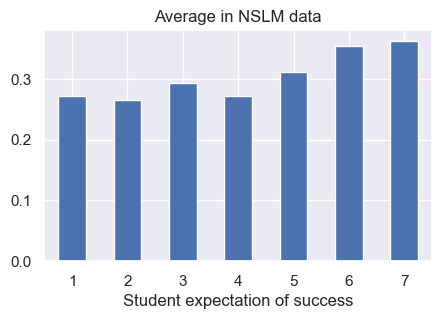
\includegraphics[scale=0.5]{img/fig-nslm-1.png}
\end{figure}
More ambitious students may be more willing to go to the seminar, leading to selection bias. How can we correct for that?

\end{frame}


%%%%%%%%%%%%%%%%%%%%%%%%%%%%%%%%%%%%%%%%%%%%%%%%%%%%%%%%%%%%%%%%%%%%%%%%%%%%%%%%
\begin{frame}[t]{Propensity Score Theorem}

Define the propensity score (or balancing score) to be:
\begin{align*}
{\color{cyan}p(X_i)} =& \mathbf{E} [D_i \vert X_i] \\
=& \sum_{d=0}^1 d \cdot \mathbf{P} (D_i = d \vert X_i) \\
=& 0 \cdot \mathbf{P} (D_i = 0 \vert X_i) + 1 \cdot \mathbf{P} (D_i = 1 \vert X_i) \\
=& {\color{Green}\mathbf{P} (D_i = 1 \vert X_i)}
\end{align*}
\textbf{Note:} the {\color{cyan}propensity score} equals the {\color{Green}probability of treatment} for binary treatments

\vspace{3ex}
Suppose the CIA holds such that $\{Y_i(0), Y_i(1)\} \perp D_i \vert X_i$. Then $\{Y_i(0), Y_i(1) \} \perp D_i \vert p(X_i)$

\vspace{3ex}\textbf{What does this mean?}
\begin{itemize}
    \item You don't need to directly control for confounders $X$ to achieve CIA
    \item Instead, it is sufficient to control for a single variable, $p(X_i)$
\end{itemize}


\end{frame}

%%%%%%%%%%%%%%%%%%%%%%%%%%%%%%%%%%%%%%%%%%%%%%%%%%%%%%%%%%%%%%%%%%%%%%%%%%%%%%%%
\begin{frame}[t]{}

{\color{DarkGray}\textbf{Propensity Score Theorem:} Given propensity score:
\begin{equation*}
    p(X_i) = \EE [D_i \vert X_i] = \PP (D_i = 1 \vert X_i)
\end{equation*}
Suppose the CIA holds such that $\{Y_i(0), Y_i(1)\} \perp D_i \vert X_i$. Then $\{Y_i(0), Y_i(1) \} \perp D_i \vert p(X_i)$
}

\vspace{3ex}
\textbf{Proof:}

First, instead of writing $\{Y_i(0), Y_i(1)\}$, we'll write $Y_i(j)$, where $j \in {0, 1}$.

\vspace{2ex}
Next, note that the conditional expectation of the treatment variable equals the conditional probability of treatment (because the treatment is binary):
\begin{align*}
    \EE [D_i \vert Y_i(j), p(X_i)] =& \sum_{d = 0}^1 d \PP (D_i = d \vert Y_i(j), p(X_i)) \\
    =& 0 \cdot \PP (D_i = 0 \vert Y_i(j), p(X_i))
    + 1 \cdot \PP (D_i = 1 \vert Y_i(j), p(X_i)) \\
    =& \PP (D_i = 1 \vert Y_i(j), p(X_i))
\end{align*}
\end{frame}



%%%%%%%%%%%%%%%%%%%%%%%%%%%%%%%%%%%%%%%%%%%%%%%%%%%%%%%%%%%%%%%%%%%%%%%%%%%%%%%%
\begin{frame}[t]{}

{\color{DarkGray}\textbf{Propensity Score Theorem:} Given propensity score:
\begin{equation*}
    p(X_i) = \EE [D_i \vert X_i] = \PP (D_i = 1 \vert X_i)
\end{equation*}
Suppose the CIA holds such that $\{Y_i(0), Y_i(1)\} \perp D_i \vert X_i$. Then $\{Y_i(0), Y_i(1) \} \perp D_i \vert p(X_i)$
}

\vspace{3ex}
\textbf{Proof:}

We want to show that:
\begin{equation*}
    {\color<2>{cyan}\EE [D_i \vert X_i, p(X_i)]}
    = 
    {\color<3>{Green}\EE [D_i \vert p(X_i)]}
\end{equation*}
\onslide<2->{
First consider the left hand side:
\begin{align*}
    {\color<2,5>{cyan}\EE [D_i \vert X_i, p(X_i)]} 
    &= \EE [D_i \vert X_i] 
    {\color<5,7>{HunterPurple}= p(X_i)}
\end{align*}
In words: $p(X_i)$ is a function of $X_i$, so conditioning on $X_i$ and $p(X_i)$ does not give any more information than conditioning on $X_i$ alone.
}

\vspace{2ex}
\onslide<3->{
    Next consider the right hand side:
    \begin{align*}
        {\color<3>{Green}\EE [D_i \vert p(X_i)] }
        % {\EE \Big[ } 
        % {\color<4>{MainBlue}\EE [}D_i \vert {\color<4>{MainBlue}X_i}, p(X_i) {\color<4>{MainBlue}]} 
        % {\Big\vert p(X_i) \Big]}
        \onslide<4->{
        &=
        {\EE \Big[ } 
        {\color<5>{cyan}
            \EE [D_i \vert {\color<4>{MainBlue}X_i}, p(X_i)]
        }
        {\Big\vert p(X_i) \Big]}
        &\because{\text{Law of iterated expectations}} \\
        }
        \onslide<5->{
        =& {\EE \Big[ } 
        {\color<5>{HunterPurple} p(X_i)}
        {\Big\vert p(X_i) \Big]}
        } \\
        \onslide<6->{
        =& {\color<7>{HunterPurple} p(X_i)}
        }
    \end{align*}
}
\onslide<7->{
    Because
    ${\color<7>{HunterPurple} p(X_i)} {\color<7>{HunterPurple}= p(X_i)}$, the statement is true.
}

\end{frame}

%%%%%%%%%%%%%%%%%%%%%%%%%%%%%%%%%%%%%%%%%%%%%%%%%%%%%%%%%%%%%%%%%%%%%%%%%%%%%%%%
\begin{frame}{}

\begin{figure}
\begin{tikzpicture}[
    node distance=1.25cm,
    every node/.style={
        draw, circle, minimum size=.85cm, align=center, inner sep=0pt
    }]

   % Nodes
  \node (X) {X};
  \node[right=of X] (pX) {$p(X)$};
  \node[right=of pX] (D) {D};
  \node[right=of D] (Y) {$Y$};

  % Arrows
  \draw[->] (X) -- (pX);
  \draw[->] (pX) -- (D);
  \draw[->] (D) -- (Y);

  % Curved arrow from X to Y
  \draw[->, bend left=40] (X) to (Y);

\end{tikzpicture}
\end{figure}
\begin{itemize}
    \item If I know what $p(X)$ is, then $X$ alone doesn't tell me anything else about what the probability of treatment is
    \item Controlling for $p(X)$ acts the same way as controlling for $X$ directly
\end{itemize}

\end{frame}

%%%%%%%%%%%%%%%%%%%%%%%%%%%%%%%%%%%%%%%%%%%%%%%%%%%%%%%%%%%%%%%%%%%%%%%%%%%%%%%%
\section[Treatment effects]{Propensity scores and treatment effects}
\miniframesoff
\begin{frame}
    \tableofcontents[currentsection]
\end{frame}
\miniframeson
%%%%%%%%%%%%%%%%%%%%%%%%%%%%%%%%%%%%%%%%%%%%%%%%%%%%%%%%%%%%%%%%%%%%%%%%%%%%%%%%

%%%%%%%%%%%%%%%%%%%%%%%%%%%%%%%%%%%%%%%%%%%%%%%%%%%%%%%%%%%%%%%%%%%%%%%%%%%%%%%%
\begin{frame}{Propensity scores and treatment effects}

How are propensity scores used in practice?
\begin{itemize}
    \item First, estimate the propensity score
    \begin{itemize}
        \item Use a parametric model, like a logit or probit model
    \end{itemize}
    \item Next generate the effect of treatment
    \begin{itemize}
        \item Match on estimated score (direct propensity score matching)
        \item OR use weighting scheme described next
    \end{itemize}
\end{itemize}

\end{frame}

%%%%%%%%%%%%%%%%%%%%%%%%%%%%%%%%%%%%%%%%%%%%%%%%%%%%%%%%%%%%%%%%%%%%%%%%%%%%%%%%
\begin{frame}{Direct propensity score matching}

Given a propensity score, $p(X_i)$, and the CIA $\{Y_i(0), Y_i(1)\} \perp D_i \vert X_i$:
\begin{align*}
    \delta_{ToT} =& \EE [Y_i(1) - Y_i(0) \vert D_i = 1] \\
    =& \EE \left[
        \EE [Y_i \vert p(X_i), D_i = 1]
        - \EE [Y_i\vert p(X_i), D_i = 0]
    \right]
\end{align*}
Just like we did for matching, you can
\begin{itemize}
    \item Stratify the sample in to values of $p(X_i)$
    \item Find treatment effects conditional on similar $p(X_i)$
    \item Weigh these treatment effects by the distribution of $p(X_i)$ conditional on treatment
\end{itemize}

\end{frame}

%%%%%%%%%%%%%%%%%%%%%%%%%%%%%%%%%%%%%%%%%%%%%%%%%%%%%%%%%%%%%%%%%%%%%%%%%%%%%%%%
\begin{frame}{Propensity score weights}

Alternative: estimate treatment effects using propensity score weights. Final equation:
\begin{equation*}
    \mathbf{E} [Y_i(1) - Y_i(0)]
    = \mathbf{E} \left[ \frac{Y_i \left[ D_i - p(X_i) \right]}{p(X_i) (1 - p(X_i))} \right] 
\end{equation*}
We'll go through the math. Motivation for this method:
\begin{itemize}
    \item Avoids the matching step
    \item The concept of inverse probability weighting is important in more advanced topics
\end{itemize}
To prove this, we'll have to prove a few interim steps

\end{frame}

%%%%%%%%%%%%%%%%%%%%%%%%%%%%%%%%%%%%%%%%%%%%%%%%%%%%%%%%%%%%%%%%%%%%%%%%%%%%%%%%
\begin{frame}[t]{}

{\color{DarkGray}
\textbf{Fact \#1:}
\begin{equation*}
    \EE \left[ \frac{Y_i D_i}{p(X_i)} \right] = \EE [Y_i(1)]
\end{equation*}
}

\vspace{2ex}
\onslide<2->{
\textbf{Proof:}
First note that \alert<5>{$D_i = D_i^2$} for $D_i = 0$ and $D_i = 1$.    

\onslide<3->{
\vspace{1ex}
Next, recall \alert<3>{$Y_i = Y_i(0) + (Y_i(1) - Y_i(0)) D_i$}:
\begin{align*}
Y_i D_i =& \alert<3>{(Y_i(0) + (Y_i(1) - Y_i(0)) D_i)} D_i \\
\onslide<4->{=& Y_i(0) D_i + (Y_i(1) - Y_i(0)) \alert<5>{D_i^2} \\}
\onslide<5->{=& Y_i(0) D_i + (Y_i(1) - Y_i(0)) \alert<5>{D_i} \\
=& Y_i(1) D_i}
\end{align*}

\onslide<6->{
Using the above equality, the conditional independence assumption, and the definition of the propensity score:
\begin{align*}
\mathbf{E} [ Y_i D_i \vert X_i ]
=& \mathbf{E} [ Y_i(1) D_i \vert X_i ]  &&\because Y_i D_i = Y_i(1) D_i \\
\onslide<7->{
=& \mathbf{E} [Y_i(1) \vert X_i ] \cdot \mathbf{E} [D_i \vert X_i ] &&\because \left. Y_i(1) \perp D_i \right\vert X_i\\}
\onslide<8->{=& \mathbf{E} [Y_i(1) \vert X_i ] p(X_i) &&\because p(X_i) = \mathbf{E} [D_i \vert X_i ]}
\end{align*}

} % \onslide<6->
} % \onslide<3->
} % \onslide<2->

\end{frame}

%%%%%%%%%%%%%%%%%%%%%%%%%%%%%%%%%%%%%%%%%%%%%%%%%%%%%%%%%%%%%%%%%%%%%%%%%%%%%%%%
\begin{frame}[t]{}

{\color{DarkGray}
\textbf{Fact \#1:}
\begin{equation*}
    \EE \left[ \frac{Y_i D_i}{p(X_i)} \right] = \EE [Y_i(1)]
\end{equation*}
}

\vspace{2ex}
\textbf{Proof: (cont.)}

\onslide<2->{  
\vspace{1ex}
We've seen:
\begin{equation*}
    \mathbf{E} [ Y_i D_i \vert X_i ] = \mathbf{E} [Y_i(1) \vert X_i ] p(X_i)
\end{equation*}

\vspace{1ex} Now we can estimate $\mathbf{E} \left[ \frac{Y_i D_i}{p(X_i)} \right]$:
\begin{align*}
\onslide<3->{
\mathbf{E} \left[ \frac{Y_i D_i}{p(X_i)} \right] =&
\mathbf{E} \left[ \mathbf{E} \left[ \left. \frac{Y_i D_i}{p(X_i)} \right\vert X_i \right] \right] 
&&\because \text{Law of iterated expectations} \\}
\onslide<4->{
=&  \mathbf{E} \left[ \frac{1}{p(X_i)} \mathbf{E} \left[  \left. Y_i D_i \right\vert X_i \right] \right] \\}
\onslide<5->{
=&  \mathbf{E} \left[ \frac{1}{p(X_i)} \mathbf{E} [Y_i(1) \vert X_i ] p(x) \right]
&&\because \mathbf{E} [ Y_i D_i \vert X_i ] = \mathbf{E} [Y_i(1) \vert X_i] p(X_i) \\}
\onslide<6->{
=&  \mathbf{E} \left[ \frac{p(X_i)}{p(X_i)} \mathbf{E} [Y_i(1) \vert X_i ] \right] \\
}
\onslide<7->{
=& \mathbf{E} [Y_i(1)]
&&\because \text{Law of iterated expectations}
}
\end{align*}


} % \onslide<2->
\end{frame}

%%%%%%%%%%%%%%%%%%%%%%%%%%%%%%%%%%%%%%%%%%%%%%%%%%%%%%%%%%%%%%%%%%%%%%%%%%%%%%%%
\begin{frame}[t]{}

{\color{DarkGray}
\textbf{Fact \#2:}
\begin{equation*}
    \mathbf{E} \left[ \frac{Y_i (1 - D_i)}{1 - p(X_i)} \right] = \mathbf{E} [Y_i(0)]
\end{equation*}
}

\vspace{2ex}
\textbf{Proof:}
Recall {$Y_i = Y_i(0) + (Y_i(1) - Y_i(0))$}, and note $D_i (1 - D_i) = 0$ for $D_i = 0$ and $D_i = 1$:
\begin{align*}
Y_i (1 - D_i) 
\onslide<2->{=& (Y_i(0) + (Y_i(1) - Y_i(0)) D_i) (1 - D_i) \\}
\onslide<3->{=& Y_i(0) (1 - D_i) + (Y_i(1) - Y_i(0)) D_i (1 - D_i) \\}
\onslide<4->{
=& Y_i(0) (1 - D_i) + (Y_i(1) - Y_i(0)) \cdot 0 \\}
\onslide<5->{
=& Y_i(0) (1 - D_i)}
\end{align*}

\onslide<6->{
Using the above equality, the conditional independence assumption, and the definition of the propensity score:
\begin{align*}
\mathbf{E} [ Y_i (1 - D_i) \vert X_i ]
=& \mathbf{E} \left[ \left. Y_i(0) (1 - D_i) \right\vert X_i \right] \\
\onslide<7->{
=& \mathbf{E} [ Y_i(0) \vert X_i ] \cdot \mathbf{E} [1 - D_i \vert X_i]
&&\because \left. Y_i(0) \perp D_i \right\vert X_i\\}
\onslide<8->{=& \mathbf{E} [ Y_i(0) \vert X_i ] (1 - p(X_i))}
\end{align*}


} % \onslide<6->
\end{frame}

%%%%%%%%%%%%%%%%%%%%%%%%%%%%%%%%%%%%%%%%%%%%%%%%%%%%%%%%%%%%%%%%%%%%%%%%%%%%%%%%
\begin{frame}{}

{\color{DarkGray}
\textbf{Fact \#2:}
\begin{equation*}
    \mathbf{E} \left[ \frac{Y_i (1 - D_i)}{1 - p(X_i)} \right] = \mathbf{E} [Y_i(0)]
\end{equation*}
}

\vspace{2ex}
\textbf{Proof (cont.):}

\vspace{1ex}
We've seen:
\begin{equation*}
    \alert<4>{\mathbf{E} [ Y_i (1 - D_i) \vert X_i ]
    = \mathbf{E} [ Y_i(0) \vert X_i ] (1 - p(X_i))}
\end{equation*}
Now we can estimate $\mathbf{E} \left[ \frac{Y_i (1 - D_i)}{1 - p(X_i)} \right]$:
\begin{align*}
\onslide<2->{
\mathbf{E} \left[ \frac{Y_i (1 - D_i)}{1 - p(X_i)} \right]
=& \mathbf{E} \left[ \mathbf{E} \left[ \left. \frac{Y_i (1 - D_i)}{1 - p(X_i)} \right\vert X_i \right] \right]
&&\because \text{Law of iterated expectations} \\}
\onslide<3->{
=& \mathbf{E} \left[ \frac{1}{1 - p(X_i)} 
\alert<4>{\mathbf{E} \left[ \left. Y_i (1 - D_i) \right\vert X_i \right]} \right] \\}
\onslide<4->{
=& \mathbf{E} \left[ \frac{1}{1 - p(X_i)} 
\alert<4>{\mathbf{E} [ Y_i(0) \vert X_i ] (1 - p(X_i))} \right] 
% &&\because \mathbf{E} [ Y_i (1 - D_i) \vert X_i ] = \mathbf{E} [ Y_i(0) \vert X_i ] (1 - p(X_i))
\\}
\onslide<5->{
=& \mathbf{E} \left[\mathbf{E} [ Y_i(0) \vert X_i ] \right] \\}
\onslide<6->{
=& \mathbf{E} [Y_i(0)] 
&&\because \text{Law of iterated expectations}}
\end{align*}


\end{frame}

%%%%%%%%%%%%%%%%%%%%%%%%%%%%%%%%%%%%%%%%%%%%%%%%%%%%%%%%%%%%%%%%%%%%%%%%%%%%%%%%
\begin{frame}{}

We've seen
\begin{equation*}
\EE \left[ \frac{Y_i D_i}{p(X_i)} \right] = \EE [Y_i(1)],
\quad \quad
    \mathbf{E} \left[ \frac{Y_i (1 - D_i)}{1 - p(X_i)} \right] = \mathbf{E} [Y_i(0)]
\end{equation*}
Average treatment effects can be estimated from:
\begin{align*}
\mathbf{E} [Y_i(1) - Y_i(0)]
=& \mathbf{E} 
\left[ 
    \frac{Y_i D_i}{p(X_i)}
    - \frac{Y_i (1 - D_i)}{1 - p(X_i)}
\right] \\
=& \mathbf{E} \left[ \frac{Y_i D_i (1 - p(X_i)) - Y_i (1 - D_i) p(X_i)}{p(X_i) (1 - p(X_i))} \right] \\
=& \mathbf{E} \left[ \frac{Y_i \left[ D_i (1 - p(X_i)) - (1 - D_i) p(X_i) \right]}{p(X_i) (1 - p(X_i))} \right] \\
=& \mathbf{E} \left[ \frac{Y_i \left[ D_i - D_i p(X_i) - p(X_i) +  D_i p(X_i) \right]}{p(X_i) (1 - p(X_i))} \right] \\
=& \mathbf{E} \left[ \frac{Y_i \left[ D_i - p(X_i) \right]}{p(X_i) (1 - p(X_i))} \right] \\
\end{align*}

\end{frame}

%%%%%%%%%%%%%%%%%%%%%%%%%%%%%%%%%%%%%%%%%%%%%%%%%%%%%%%%%%%%%%%%%%%%%%%%%%%%%%%%
\begin{frame}{}

Horvitz-Thompson Propensity score weighting:
\begin{equation*}
    \mathbf{E} [Y_i(1) - Y_i(0)]
    = \mathbf{E} \left[ \frac{Y_i \left[ D_i - p(X_i) \right]}{p(X_i) (1 - p(X_i))} \right]
\end{equation*}
\begin{itemize}
    \item Uses propensity score weighting to recover average treatment effects
    \item Using the propensity score rather than identification by conditioning on $X$ is a useful empirical strategy when $X$ is high-dimensional and $p(X)$ is available (or can be approximated accurately)
    \item MHE shows how this can be considered similar to the regression estimator
\end{itemize}


\end{frame}




%%%%%%%%%%%%%%%%%%%%%%%%%%%%%%%%%%%%%%%%%%%%%%%%%%%%%%%%%%%%%%%%%%%%%%%%%%%%%%
\section[Extensions]{Important extensions}
\miniframesoff
\begin{frame}
    \tableofcontents[currentsection]
\end{frame}
\miniframeson
%%%%%%%%%%%%%%%%%%%%%%%%%%%%%%%%%%%%%%%%%%%%%%%%%%%%%%%%%%%%%%%%%%%%%%%%%%%%%%

%%%%%%%%%%%%%%%%%%%%%%%%%%%%%%%%%%%%%%%%%%%%%%%%%%%%%%%%%%%%%%%%%%%%%%%%%%%%%%
\begin{frame}{Inverse Probability of Treatment Weighting}
We've seen:
\begin{equation*}
{\color<6>{DarkGray}\EE \left[ \frac{{\color<2>{cyan}Y_i D_i}}{{\color<3-4>{cyan} p(X_i)}} \right] = \EE [Y_i(1)]},
\quad \quad
{\color<2-5>{DarkGray}\mathbf{E} \left[ \frac{Y_i (1 - D_i)}{1 - p(X_i)} \right] = \mathbf{E} [Y_i(0)]}
\end{equation*}
Consider the first element:
\begin{itemize}
    \onslide<2->{\item {\color<2>{cyan} $Y_i D_i$}: Isolates $Y_i$ that are treated}
    \onslide<3->{\item {\color<3-4>{cyan} $p(X_i)$}: Inverse probability of being treated
    \onslide<4->{
    \begin{itemize}
        \item Probabilities are between 0 and 1
        \item Low probability events $\implies$ inverse probability high
        \begin{align*}
            p(X) = 0.1 = \frac{1}{10} \implies& \frac{1}{p(X)} = \frac{1}{1/10} = 10
        \end{align*}
        \item High probability events $\implies$ inverse probability low
        \begin{align*}
p(X) = 0.8 = \frac{4}{5} \implies& \frac{1}{p(X)} = \frac{1}{4/5} = 1.25
        \end{align*} 
    \end{itemize}
    \onslide<5->{
    \item Treated observations with a low $p(X)$ probably look more like the untreated. Therefore, they receive greater weight. Vice versa for the untreated
    }
    }}
\end{itemize}
\onslide<6->{The same reasoning applies to the second element}

\vspace{3ex}
\onslide<7->{IPTW: valuable in a clinical setting to generate balanced data}

\end{frame}

%%%%%%%%%%%%%%%%%%%%%%%%%%%%%%%%%%%%%%%%%%%%%%%%%%%%%%%%%%%%%%%%%%%%%%%%%%%%%%%%
\begin{frame}{Structural model and connection to machine learning}

Note: the following is from \emph{Business Data Science} by Matt Taddy, Chapter 6

\vspace{3ex}
Consider a common structural model:
\begin{align*}
    Y &= D \gamma + X^\prime \beta + \epsilon, \quad \epsilon \vert D, X = 0 \\
    D &= X^\prime \tau + v, \quad v \vert X = 0
\end{align*}
Note:
\begin{itemize}
    \item $\epsilon \vert D, X = 0$ and $v \vert X = 0$ encode CIA
\end{itemize}
Two-step \textbf{linear treatment effects (LTE)} model
\begin{itemize}
    \item First estimate treatment $D_i$
    \item Then estimate treatment effects $\gamma$
\end{itemize}
Dimensionality starts to matter here
\begin{itemize}
    \item If $n$ (number of observations) are much greater than $p$ (number of $X$ variables), you can use regression models
    \item If you don't have $n>>p$, traditional methods break down
\end{itemize}
\end{frame}

%%%%%%%%%%%%%%%%%%%%%%%%%%%%%%%%%%%%%%%%%%%%%%%%%%%%%%%%%%%%%%%%%%%%%%%%%%%%%%%%
\begin{frame}{Estimation of LTE}
Structural model:
\begin{align*}
    Y &= D \gamma + X^\prime \beta + \epsilon, \quad \epsilon \vert D, X = 0 \\
    D &= X^\prime \tau + v, \quad v \vert X = 0
\end{align*}
Estimation procedure:
\begin{enumerate}
    \item Estimate $\EE [D \vert X] = X^\prime \tau$. Collect fitted values
    $\hat{D} = X^\prime \hat{\tau}$
    \item Estimate:
    \begin{equation*}
        \EE [Y \vert X, D] = \hat{D} \psi + D \gamma + X^\prime \beta
    \end{equation*}
\end{enumerate}
The $\psi$ is the treatment effect of $D$ on $Y$.

\end{frame}

%%%%%%%%%%%%%%%%%%%%%%%%%%%%%%%%%%%%%%%%%%%%%%%%%%%%%%%%%%%%%%%%%%%%%%%%%%%%%%%%
\begin{frame}{LTE and propensity score matching}

Structural model in propensity score models:
\begin{align*}
    Y &= D \gamma + X^\prime \beta + \epsilon, \quad \epsilon \vert D, X = 0 \\
    D &\sim \text{Bernoulli}\left( p(X) \right) \\
    p(X) &= \frac{e^{X^\prime \tau}}{1 + e^{X^\prime \tau}}
\end{align*}
\begin{itemize}
    \item $D$ is modeled from a Bernoulli distribution (i.e. coin toss) with probability $p$
    \item The probability that $D=1$ is modeled using a \textbf{logistic regression}
\end{itemize}
Once you estimate the propensity score $p(X)$, you can find treatment effects by:
\begin{enumerate}
    \item Fitting the linear regression: $\EE [Y \vert D, \hat{p} (X)] = \alpha + D \gamma + \hat{p}(X) \psi$
    \item Constructing propensity score weighting estimates: $\EE \left[ \left. \frac{Y}{\hat{p(X)}} \right\vert D \right] = \alpha + D \gamma$ 
    \item Matching 
\end{enumerate}

\end{frame}

%%%%%%%%%%%%%%%%%%%%%%%%%%%%%%%%%%%%%%%%%%%%%%%%%%%%%%%%%%%%%%%%%%%%%%%%%%%%%%%%
\begin{frame}{}

Hahn (1998) shows there is a cost to propensity score matching in terms of asymptotic efficiency
\begin{itemize}
    \item What is the advantage of, say, controlling for propensity score instead of controlling for covariates in a regression?
\end{itemize}

\vspace{2ex}
MHE : ``An essential element of  propensity score methods is the use of prior knowledge for dimension reduction. The statistical payoff is an improvement in finite sample behavior. If you're not prepared to smooth, restrict, or otherwise reduce the dimensionality of the matching problem in a manner that has real empirical consequences, the you might as well go for full covariate matching or saturated regression control.''
\begin{itemize}
    \item This is very prescient! Now, in the era of big data, dimensionality reduction is key
    \item Propensity scores have a new value in double-robust machine learning; see chapter 9 of \url{https://chapters.causalml-book.org/CausalML_chap_9.pdf}
\end{itemize}

\end{frame}

% %%%%%%%%%%%%%%%%%%%%%%%%%%%%%%%%%%%%%%%%%%%%%%%%%%%%%%%%%%%%%%%%%%%%%%%%%%%%%%%%
% \begin{frame}{}

% Doudbly robust?

% \end{frame}





%%%%%%%%%%%%%%%%%%%%%%%%%%%%%%%%%%%%%%%%%%%%%%%%%%%%%%%%%%%%%%%%%%%%%%%%%%%%%%
\section[Logit models]{Logistic regression}
\miniframesoff
\begin{frame}
    \tableofcontents[currentsection]
\end{frame}
\miniframeson
%%%%%%%%%%%%%%%%%%%%%%%%%%%%%%%%%%%%%%%%%%%%%%%%%%%%%%%%%%%%%%%%%%%%%%%%%%%%%%

%%%%%%%%%%%%%%%%%%%%%%%%%%%%%%%%%%%%%%%%%%%%%%%%%%%%%%%%%%%%%%%%%%%%%%%%%%%%%%%%
\begin{frame}{Why logistic regression}

\begin{itemize}
    \item We have to use some estimation procedure to predict propensity scores $p(X)$
    \item Logistic regression is a common method
    \item Quick review of logistic regression and generalized linear models
\end{itemize}

\end{frame}

%%%%%%%%%%%%%%%%%%%%%%%%%%%%%%%%%%%%%%%%%%%%%%%%%%%%%%%%%%%%%%%%%%%%%%%%%%%%%%%%
\begin{frame}{Linear regression}

Assume we have data $\{y_i, x_{1i}, x_{2i}, \dots, x_{ki}\} = \{y_i, \mathbf{x}_i\}$. A linear regression model takes the form:
\begin{equation*}
    y_i = \beta_0 + \beta_1 x_{1i} + \beta_2 x_{2i} + \dots + \beta_k x_{ki} + \epsilon_i = \mathbf{x}_i^T \boldsymbol{\beta} + \epsilon_i, \quad i = 1, \dots, n
\end{equation*}
We can stack these equations for all $n$ equations in the data:
\begin{equation*}
    \mathbf{y} = \mathbf{X} \boldsymbol{\beta} + \boldsymbol{\epsilon}
\end{equation*}
To estimate this model using least squares, find the coefficient matrix $\boldsymbol{\beta}$ that minimizes the sum of squared residuals:
\begin{equation*}
    \hat{\boldsymbol{\beta}} = \arg \min_{\boldsymbol{\beta}} 
    = \sum_{i = 1}^n \left( y_i - \sum_{j=1}^K x_{ji} \beta_j \right)^2
\end{equation*}
A more math-y way of saying this using norm notation:
\begin{equation*}
    \hat{\boldsymbol{\beta}} = \arg \min_{\boldsymbol{\beta}} 
    \left\vert \left\vert
    \mathbf{y} - \mathbf{X} \boldsymbol{\beta}
    \right\vert\right\vert^2
\end{equation*}
\begin{itemize}
    \item Just think about the norm notation $\vert \vert \cdot \vert \vert$ communicating size in a multidimensional space
\end{itemize}
\end{frame}

%%%%%%%%%%%%%%%%%%%%%%%%%%%%%%%%%%%%%%%%%%%%%%%%%%%%%%%%%%%%%%%%%%%%%%%%%%%%%%%%
\begin{frame}{Limitations of linear model}

We are trying to predict treatment, $D_i$
\begin{itemize}
    \item Always takes on values equal to zero or 1
    \item Do we really want a linear model?
\end{itemize}
Consider data on hours studied and passing/failing a test ($D=1$ implies a student passed)

\begin{figure}
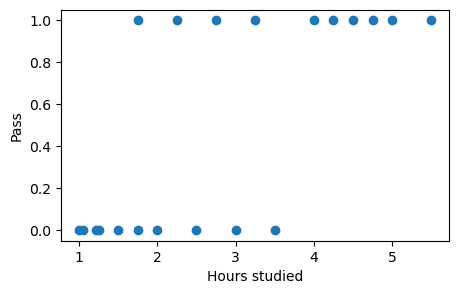
\includegraphics[scale=0.5]{img/fig-scatter.png}
\end{figure}

\end{frame}

%%%%%%%%%%%%%%%%%%%%%%%%%%%%%%%%%%%%%%%%%%%%%%%%%%%%%%%%%%%%%%%%%%%%%%%%%%%%%%%%
\begin{frame}{OLS}

We could estimate using a linear model:

\begin{figure}
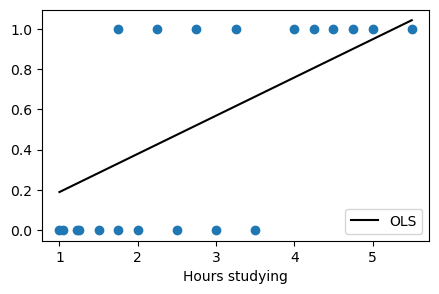
\includegraphics[scale=0.5]{img/fig-ols.png}
\end{figure}
\begin{itemize}
    \item Line isn't a great fit
\end{itemize}

\end{frame}

%%%%%%%%%%%%%%%%%%%%%%%%%%%%%%%%%%%%%%%%%%%%%%%%%%%%%%%%%%%%%%%%%%%%%%%%%%%%%%%%
\begin{frame}{Logit}

We could estimate using a linear model:

\begin{figure}
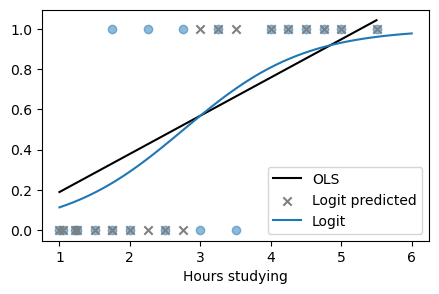
\includegraphics[scale=0.5]{img/fig-ols_logit.png}
\end{figure}
\begin{itemize}
    \item Logistic line is a better fit
    \item Less important: output is binary
\end{itemize}

\end{frame}


\end{document}